\documentclass{article}

\usepackage[a4paper, margin=3cm]{geometry}
\usepackage{float}
\usepackage{algorithm2e}
\usepackage{graphicx}
\usepackage{amsmath}
\usepackage{amssymb}
\usepackage{multicol}

\title{Lesson 2 : Problem Solving Paradigms}
\author{CPC UTEC - Lecturers Notes}


\begin{document}

\maketitle

\setlength{\parindent}{0mm}

\textbf{Scope \& Objectives:}
\begin{itemize}
	\item Have a formal understanding of Big-Oh notation.
	\item Learn about the popular problem solving paradigms.
	\item Understand Complete Search and brute force.
\end{itemize}

\setlength{\parskip}{4mm}

\section{Algorithmic Analysis}

\textit{Big-Oh} notation is a tool we can use to measure how the complexity of our solution scales as the input of our program grows. This is done by measuring how our complexity compares to other functions as the input size goes to infinity. For this reason this is know as \textit{Asymptotic Analysis}.

Formally, we can define Big-Oh notation as:
$$f(n) = O(g(n)) \longleftrightarrow f(n) \leq kg(n)$$
$$\text{Where } n > n_0, \; k > 0 \text{ and } n_0 \in \mathbb{R}$$

This definition might seem complex but is very simple to understand. We can use the aid of the following graph:

\begin{figure}[H]
	\centering
	\includegraphics[width=0.5\linewidth]{images/bigoh}
	\caption{Graphical understanding of Big-Oh}
\end{figure}

First of all we must understand that $O(g(n))$ is not a function but a family (or set) of functions. For this reasons many believe that the `$\in$' symbol would be more appropriate than the `=' symbol. Therefore, it is a good idea to read the `=' sign as \textit{belongs} or \textit{is in}.

\section{Problem Solving Paradigms}

\subsection{Paradigm vs Algorithm}

\begin{multicols}{2}
	\raggedcolumns
	\centering \textbf{Algorithm}
	\begin{itemize}
		\item Solves a specific problem.
		\item Gives steps and instructions.
	\end{itemize}

	\columnbreak

	\centering \textbf{Paradigm}
	\begin{itemize}
		\item Solves a family of problems.
		\item Gives ideas and methodologies.
		\item Is a conceptual framework for problem solving.
	\end{itemize}
\end{multicols}

\subsection{Popular Paradigms}

\begin{figure}[H]
	\centering
	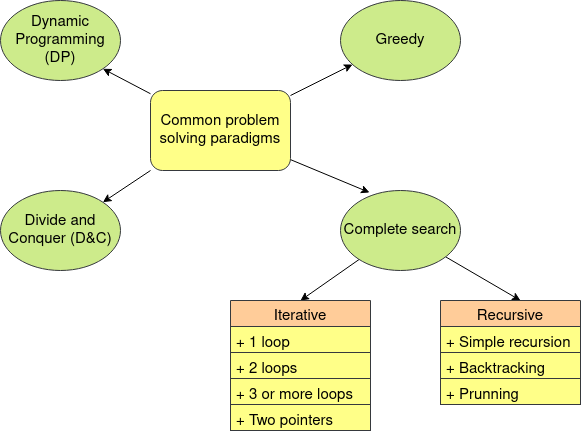
\includegraphics[width=0.7\linewidth]{images/programming-paradigms}
	\caption{Popular problem solving paradigms.}
\end{figure}

\section{Complete Search}

Most competitive programming problems (and most problems in general) can be solved by listing all the possible solutions and checking each of them until we find the correct one. This method of problems solving in which we exhaustively check all possible solutions is called \textit{complete search}.

This paradigm is extremely important as we can almost always find a complete search solutions to any given problem (even though this solution will probably violate the time constrains). Being good at designing complete search solutions is extremely important to learn the other problems solving paradigms and understanding the importance of optimizations.

\subsection{Key Terms} 

\begin{itemize}
	\item \textbf{Solution-Space:} All the candidate or possible solutions there are.
	\item \textbf{Brute Force:} Iterative complete search.
	\item \textbf{Fixing:} Assuming a \textit{variable} has a constant value.
\end{itemize}

\subsection{Example: Number of solutions}

Lets consider the following problem. Given the positive integers $a$, $b$, $c$ and $d$, find how many solutions the equation $x + y + z = d$ has, given that $x, y, z \in \mathbb{N}^+$, $x \leq a$, $y \leq b$ and $z \leq c$.

A first approach for solving this problem is to fix the values of $x$, $y$ and $z$. We can then find the value of $x + y + z$ and check if it equals $d$.

\begin{algorithm}
	\SetAlgoNoEnd
	$cnt \gets 0$\;
	\For{$x \gets 1$ \KwTo $a$}{
		\For{$y \gets 1$ \KwTo $b$}{
			\For{$z \gets 1$ \KwTo $c$}{
				\If{$x + y + z = d$}{
					$cnt \gets cnt + 1$\;
				}
			}
		}
	}
	\Return $cnt$\;
\end{algorithm}

It is simple to see that this solution has a complexity of $O(n^3)$. In general, for complete search our time complexity can be estimates as:

$$T(n) = |\text{Solution Space}| \times \text{time to check a solution}$$

In this example we take $O(1)$ to check each candidate solution, but we visit $O(n^3)$ possible solutions, giving the total complexity of $O(n^3)$. Can we improve this solution?

One important observation is to realize that if we fix the values of $a$ and $b$, then we can re-write the equation as: $z = d - x - y$. This means that for every pair of values $(x, y)$, there exists a single possible value of $z$ that can satisfy the equation. Now we all have to do is verify that the value of $z$ is valid.

\begin{algorithm}
	\SetAlgoNoEnd
	$cnt \gets 0$\;
	\For{$x \gets 1$ \KwTo $a$}{
		\For{$y \gets 1$ \KwTo $b$}{
			$z \gets d - x - y$\;
			\If{$1 \leq z \leq c$}{
				$cnt \gets cnt + 1$\;
			}
		}
	}
	\Return $cnt$\;
\end{algorithm}

Our time taken to verify each solution is still $O(1)$, however the size of our solution space is now $O(n^2)$. This drastically improves the solutions complexity, taking it from $O(n^3)$ to $O(n^2)$. Further improvements can be done to make in order to find the answer in $O(n)$ time or faster.

The most important takeaway of this example should be that a brute force algorithm is not necessarily a dumb or easy algorithm, many time brute force solutions need to be tightly optimized in order to yield a correct solution that works within the time constrains.

\end{document}
